\chaptertitle{第一章\quad 集合基础}

为什么讲组合数学要先讲集合？因为组合数学研究的对象是"一组东西"。不管是数排列的方法、画图的顶点和边，还是讨论哪些情况可能发生，我们都需要一种精确的方式来描述"一组东西"以及它们之间的相互关系。集合就是这种语言。学完本章，你将能够用集合的语言来表述和解决简单的组合问题。

\sectiontitle{1.1\quad 集合与元素}

先看三个句子：
\begin{itemize}
\item "第一排的同学们"
\item "书包里的文具"
\item "小于$10$的正整数"
\end{itemize}

我们把这些对象看作一个整体。在数学中，我们把这种"确定的对象汇集在一起"形成的整体称为\textbf{集合}。集合中的每个对象称为它的\textbf{元素}。

\begin{example}
判断以下哪些可以构成集合：
(1) 班里个子高的同学。
(2) $\{1,2,3,4,5\}$。
(3) 世界上跑得很快的人。
\end{example}
\begin{solution}
(1) 不能——"个子高"没有明确标准，$1.7$m算高还是$1.8$m算高？元素不确定。\\
(2) 能——五个数字是确定的。\\
(3) 不能——"很快"没有明确标准。
\end{solution}

我们用大写字母表示集合（如$A,B,C$），用小写字母表示元素（如$a,b,c$）。
如果$a$是集合$A$的元素，记作$a\in A$（读作"$a$属于$A$"）；
如果不是，记作$a\notin A$（读作"$a$不属于$A$"）。

有些数集在数学中非常常用，有固定的记号：
\begin{center}
\begin{tabular}{c|c}
记号 & 含义 \\ \hline
$\mathbb N$ & 自然数集$\{0,1,2,3,\dots\}$ \\
$\mathbb Z$ & 整数集$\{\dots,-2,-1,0,1,2,\dots\}$ \\
$\mathbb Q$ & 有理数集（可以写成分数的数） \\
$\mathbb R$ & 实数集（所有数）
\end{tabular}
\end{center}

\begin{example}
判断正误：
(1) $2\in\mathbb N$ \qquad (2) $0.5\in\mathbb Z$ \qquad
(3) $-3\in\mathbb Z$ \qquad (4) $\sqrt2\in\mathbb Q$
\end{example}
\begin{solution}
(1) 真——$2$是自然数。\qquad
(2) 假——$0.5$不是整数。\\
(3) 真——$-3$是整数。\qquad
(4) 假——$\sqrt2$不能写成分数，不是有理数。
\end{solution}

\begin{exercise}
\item 判断以下哪些可以构成集合：
(1) $\{a,b,c,d\}$\quad (2) 班里跑得快的同学\quad (3) 小于$10$的质数
\item 用$\in$或$\notin$填空：
(1) $0\;\underline{\quad}\;\mathbb N$\quad (2) $\frac12\;\underline{\quad}\;\mathbb Z$\quad
(3) $\pi\;\underline{\quad}\;\mathbb R$
\end{exercise}

\sectiontitle{1.2\quad 集合的表示法}

集合有三种表示方法。

\textbf{列举法}——把元素一一写在大括号里。

\begin{example}
用列举法表示：
(1) 大于$2$且小于$7$的整数。
(2) 方程$x^2-5x+6=0$的根。
\end{example}
\begin{solution}
(1) $\{3,4,5,6\}$\qquad (2) $x^2-5x+6=0$的解是$x=2$或$x=3$，所以$\{2,3\}$。
\end{solution}

\textbf{描述法}——用元素满足的条件来表示。形式为$\{x\mid x\text{满足的条件}\}$。

\begin{example}
用描述法表示：
(1) 大于$5$的偶数。
(2) $\{1,4,9,16,25\}$。
\end{example}
\begin{solution}
(1) $\{x\mid x>5,\ x\text{是偶数}\}$。\\
(2) 观察模式：$1=1^2,4=2^2,9=3^2,16=4^2,25=5^2$，所以$\{x\mid x=n^2,n\in\mathbb N,1\le n\le5\}$。
\end{solution}

\textbf{Venn图}——用封闭曲线表示集合，直观展示元素与集合的关系。

\begin{example}
用Venn图表示集合$A=\{1,2,3\}$。
\end{example}
\begin{solution}
\begin{center}
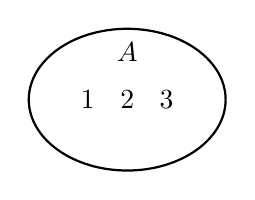
\begin{tikzpicture}[scale=0.5]
\draw[thick] (0,0) ellipse (2.5 and 1.8);
\node at (0,1.2) {$A$};
\node at (-1,0) {$1$};
\node at (0,0) {$2$};
\node at (1,0) {$3$};
\end{tikzpicture}
\end{center}
\end{solution}

\begin{exercise}
\item 用列举法表示：
(1) $\{x\in\mathbb N\mid x<6\}$\quad (2) $\{x\mid x^2-9=0\}$
\item 用描述法表示大于$0$且小于$1$的有理数。
\item 画Venn图表示集合$A=\{a,b,c,d\}$。
\end{exercise}

\sectiontitle{1.3\quad 子集与集合的运算}

\textbf{子集}：如果集合$A$的每个元素都在集合$B$中，就说$A$是$B$的\textbf{子集}，记作$A\subseteq B$。
如果$A\subseteq B$且$A\neq B$，就说是\textbf{真子集}，记作$A\subsetneq B$。
空集$\varnothing$（不含任何元素的集合）是任何集合的子集。

\begin{example}
$A=\{1,2\}$，写出$A$的所有子集。
\end{example}
\begin{solution}
子集：$\varnothing$、$\{1\}$、$\{2\}$、$\{1,2\}$，一共$4$个。\\
真子集$3$个（去掉自身）。
\end{solution}

一个$n$个元素的集合有多少个子集？我们先看几个具体例子再找规律。

\begin{center}
\begin{tabular}{c|c|c}
集合 & 元素个数$n$ & 子集个数 \\ \hline
$\varnothing$ & $0$ & $1$ \\
$\{a\}$ & $1$ & $2$ \\
$\{a,b\}$ & $2$ & $4$ \\
$\{a,b,c\}$ & $3$ & $8$
\end{tabular}
\end{center}

\begin{example}
观察上表，你发现子集个数与$n$之间有什么关系？
\end{example}
\begin{solution}
$n=0$时子集$1=2^0$，$n=1$时$2=2^1$，$n=2$时$4=2^2$，$n=3$时$8=2^3$。
所以$n$个元素的集合有$2^n$个子集（包括空集和自身）。
\end{solution}

$n$个元素的集合有$2^n$个子集，$2^n-1$个真子集。

\begin{center}
\begin{tikzpicture}[scale=0.5]
\draw[thick] (0,0) ellipse (2.5 and 2);
\node at (0,1.6) {$B$};
\draw[thick,fill=lightblue] (-0.3,-0.3) ellipse (1.3 and 1);
\node at (-0.3,1) {$A$};
\node at (0,-2.2) {$A\subseteq B$};
\end{tikzpicture}
\end{center}

\textbf{交集}与\textbf{并集}：给定两个集合$A$和$B$，
\begin{itemize}
\item 交集$A\cap B=\{x\mid x\in A\text{且}x\in B\}$——公共部分。
\item 并集$A\cup B=\{x\mid x\in A\text{或}x\in B\}$——合起来。
\end{itemize}

\begin{example}
$A=\{1,2,3,4\}$，$B=\{3,4,5,6\}$，求$A\cap B$和$A\cup B$。
\end{example}
\begin{solution}
$A\cap B=\{3,4\}$（公共元素）。\\
$A\cup B=\{1,2,3,4,5,6\}$（全部合起来，重复只写一次）。
\end{solution}

\begin{center}
\begin{tikzpicture}[scale=0.5]
\draw[thick] (-0.8,0) ellipse (1.8 and 1.5);
\draw[thick] (0.8,0) ellipse (1.8 and 1.5);
\begin{scope}
\clip (-0.8,0) ellipse (1.8 and 1.5);
\fill[lightblue] (0.8,0) ellipse (1.8 and 1.5);
\end{scope}
\node at (-1.5,1.2) {$A$};
\node at (1.5,1.2) {$B$};
\node at (0,0) {$A\cap B$};
\end{tikzpicture}
\qquad
\begin{tikzpicture}[scale=0.5]
\draw[thick,fill=lightblue] (-0.8,0) ellipse (1.8 and 1.5);
\draw[thick,fill=lightblue] (0.8,0) ellipse (1.8 and 1.5);
\node at (-1.5,1.2) {$A$};
\node at (1.5,1.2) {$B$};
\node at (0,-2.2) {$A\cup B$};
\end{tikzpicture}
\end{center}

\textbf{补集}：在全集$U$中，不属于$A$的元素组成的集合叫$A$的补集，记作$\complement_UA$。
$\complement_UA=\{x\mid x\in U\text{且}x\notin A\}$。

\begin{example}
$U=\{1,2,3,4,5,6,7\}$，$A=\{2,3,5,7\}$，求$\complement_UA$。
\end{example}
\begin{solution}
把$U$中去掉$A$中的元素：$\complement_UA=\{1,4,6\}$。
\end{solution}

\textbf{集合的计数关系}：
对于两个有限集合$A$和$B$，它们并集的元素个数满足：
\[
|A\cup B| = |A| + |B| - |A\cap B|
\]

\begin{example}
全班$50$人，喜欢数学的$30$人，喜欢物理的$25$人，两门都喜欢的$15$人。求两门都不喜欢的人数。
\end{example}
\begin{solution}
喜欢数学或物理的人数：$|A\cup B| = 30 + 25 - 15 = 40$人。\\
两门都不喜欢的人数：$50 - 40 = 10$人。
\end{solution}

\textbf{德摩根定律}（用实例验证）：
\[
\complement_U(A\cup B) = (\complement_UA) \cap (\complement_UB), \qquad
\complement_U(A\cap B) = (\complement_UA) \cup (\complement_UB)
\]

\begin{example}
$U=\{1,2,3,4,5,6\}$，$A=\{2,4,6\}$，$B=\{4,5,6\}$，验证德摩根定律。
\end{example}
\begin{solution}
$A\cup B=\{2,4,5,6\}$，$\complement_U(A\cup B)=\{1,3\}$。\\
$\complement_UA=\{1,3,5\}$，$\complement_UB=\{1,2,3\}$，$(\complement_UA)\cap(\complement_UB)=\{1,3\}$。\\
两者相等，成立。第二式同理。
\end{solution}

\begin{exercise}
\item $A=\{1,2,3\}$，写出$A$的所有子集和真子集。
\item $A=\{1,2,3,4,5\}$，$B=\{4,5,6,7\}$，求$A\cap B$，$A\cup B$。
\item $U=\{1,2,\dots,10\}$，$A=\{2,4,6,8,10\}$，求$\complement_UA$。
\item 某班$40$人，喜欢语文的$25$人，喜欢英语的$20$人，两门都喜欢的有$10$人。求两门都不喜欢的人数。
\end{exercise}

\sectiontitle{本章小结}

集合是组合数学的语言基础。本章的核心概念：集合与元素（$\in$、$\notin$）、三种表示法（列举、描述、Venn图）、子集与真子集（$2^n$个）、集合运算（交$\cap$、并$\cup$、补$\complement$）、德摩根定律。集合的计数公式$|A\cup B|=|A|+|B|-|A\cap B|$将在第六章容斥原理中推广到$n$个集合。

\sectiontitle{课后练习}

\subsection*{A组\quad 基础巩固}

\begin{exercise}
\item 用列举法表示：$\{x\in\mathbb Z\mid -2\le x<4\}$。
\item 用描述法表示偶数集合。
\item $A=\{1,3,5,7,9\}$，$B=\{3,5,11,13\}$，求$A\cap B$和$A\cup B$。
\item $n$个元素的集合有多少个真子集？
\item $U=\{a,b,c,d,e\}$，$A=\{a,c,e\}$，求$\complement_UA$。
\end{exercise}

\subsection*{B组\quad 挑战提升}

\begin{exercise}
\item 证明$|A\cup B\cup C| = |A|+|B|+|C|-|A\cap B|-|B\cap C|-|C\cap A|+|A\cap B\cap C|$（提示：画Venn图）。
\item 某班有$45$人，其中$30$人喜欢音乐，$28$人喜欢体育，$22$人喜欢美术，$15$人既喜欢音乐又喜欢体育，$12$人既喜欢音乐又喜欢美术，$10$人既喜欢体育又喜欢美术，$5$人三样都喜欢。问有多少人三样都不喜欢？
\item 是否存在一个集合，它的元素个数等于它的子集个数？如果存在，请举例。
\end{exercise}

\vfill
\noindent\rule{\textwidth}{0.4pt}
本章练习答案请参见书末附录。
